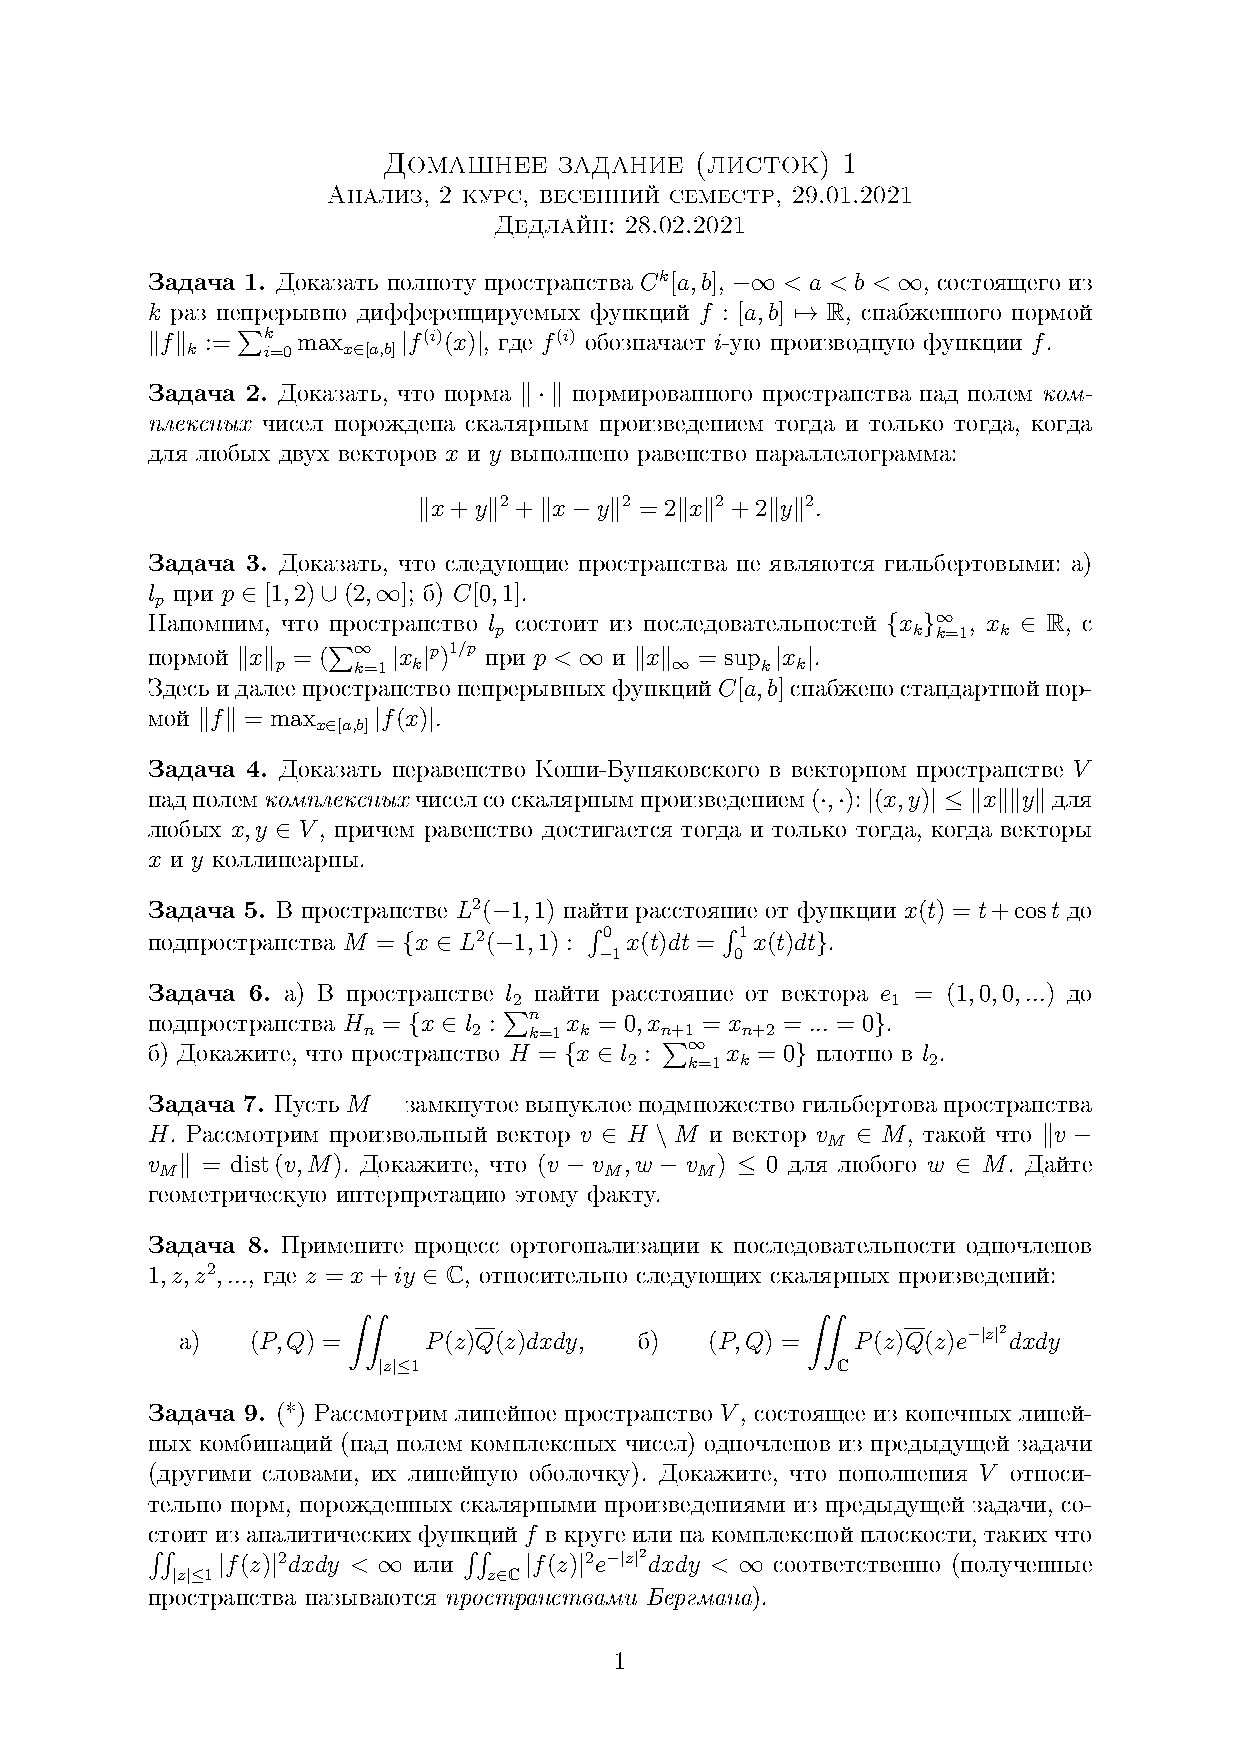
\includepdf[scale=1,pages=1-2]{Tasks/Listok1_2021.pdf}
\newpage
\section*{Решения}
\subsection*{Задача 1}
	Рассмотрим последовательность $\{f_i\}$ из $C^k [a,b]$, все положительноые пределы $\lim_i f_i^{(j)}(x)$ существуют для $j \in [0,k]$ и равномерно непрерывны. Необходимо показать что $\lim_i f^{(j)}$ дифференцируемо и производная имеет вид $\lim_i f^{(j+1)}$. Тогда покажем что для последовательности $f_n$ из $C^{1}[a,b]$ с поточечными пределами $f(x) = \lim_n f_n(x)$ и $g(x) = \lim_n f_n'(x)$ выполнено равенство $f'(x) = g(x)$. По теореме Ньютона-Лейбница для любого $i$:
	\begin{gather*}
		f_i(x) - f_i(a) = \int_{a}^{x} f_i'(t)dt
	\end{gather*}
	Тогда так как $f_i'$ поточечно сходится к $g(x)$, то для $\varepsilon > 0$ существует $i_0$ такое что $|f_i'(t) - g(t)| < \varepsilon$ для $i \geqslant i_0$ и для всех $t$. Тогда
	\begin{gather*}
		\left|\int_a^x f_i(t)dt - \int_a^x g(t)dt \right| \leqslant
		\int_a^x |f_i'(t) - g(t)|dt \leqslant
		\varepsilon \cdot |x - a| \to 0\\
		\lim_i f_i(x) - f_i(a) =
		\lim_i \int_a^x f_i'(t)dt =
		\int_a^x g(t)dt
	\end{gather*}
	Откуда $f' = g$
\vskip 0.4in


\subsection*{Задача 2}
	Пусть $||\cdot|| = \sqrt{\langle \cdot, \cdot \rangle}$, тогда
	\begin{gather*}
		\langle u+v, u+v \rangle + \langle u-v, u-v\rangle 
		= (||u||^2 + 2\langle u,v \rangle + ||v||^2) + (||u||^2 - 2\langle u,v \rangle + ||v||^2)
		= 2||u||^2 + 2||v||^2
	\end{gather*}
	
	Пусть $||\cdot||$ удовлетворяет
	\begin{gather*}
		2||u||^2 + 2||v||^2 = ||u + v||^2 + ||u - v||^2
	\end{gather*}
	и
	\begin{gather*}
		\langle x,y \rangle = \frac{1}{4}(||x + y||^2 - ||x - y||^2)
	\end{gather*}
	Заметим, что $\langle x,y \rangle = \langle y,x \rangle$ и $||x|| = \sqrt{\langle x,x \rangle}$.\\
	Далее покажем, что $(x,y) \to \langle x,y \rangle$ непрерывна, это следует из того, что сложение и вычитание $||\cdot||$-непрерывны, норма сама непрерывна, а также суммы и композиции непрерывных функций непрерывны.
	\vskip 0.1in
	Докажем что $\langle x+y, z \rangle = \langle x,z \rangle + \langle y,z \rangle$
	\begin{gather*}
		2||x + z||^2 + 2||y||^2 = ||x + y + z||^2 + ||x - y + z||^2\\
		||x + y + z||^2 = 
		2||x + z||^2 + 2||y||^2 - ||x - y + z||^2 =
		2||y + z||^2 + 2||x||^2 - ||y - x + z||^2\\
		||x + y + z||^2 = ||x||^2 + ||y||^2 + ||x + z||^2 + ||y + z||^2 - \frac{1}{2}||x - y + z||^2 - \frac{1}{2}||y - x + z||^2\\
		||x + y - z||^2 = ||x||^2 + ||y||^2 + ||x - z||^2 + ||y - z||^2 - \frac{1}{2}||x - y - z||^2 - \frac{1}{2}||y - x - z||^2\\
		\langle x+y, z\rangle = 
		\frac{1}{4}(||x + y + z||^2 - ||x + y - z||^2)\\
		= \frac{1}{4}(||x + z||^2 - ||x - z||^2) + \frac{1}{4}(||y + z||^2 - ||y - z||^2)\\
		= \langle x,z \rangle + \langle y,z \rangle
	\end{gather*}
	Теперь докажем что $\langle \lambda x,y \rangle = \lambda \langle x,y \rangle$\\
	Это очевидно выполнено для $\lambda = -1$ и по индукции $\langle \lambda x,y \rangle = \lambda \langle x,y \rangle$ для всех $\lambda \in \mathbb{N}$, рассмотрим $\lambda = \frac{p}{q},\ p,q \in \mathbb{Z},\ q \ne 0$ и $x'= \frac{x}{q}$.
	\begin{gather*}
		q \langle \lambda x, y \rangle = q\langle px', y\rangle = p\langle qx', y \rangle = p\langle x, y\rangle
	\end{gather*}
	Разделив на $q$ получим требуемое. То есть для фиксированных $x,y$ непрерывная функция $t \mapsto \frac{1}{t}\langle tx, y \rangle$ определена на $\mathbb{R} \backslash \{0\}$, то есть $\langle x,y \rangle$ на всех $t \in \mathbb{Q}\backslash \{0\}$, случай $\lambda = 0$ тривиален.
	\vskip 0.1in
	Определим $\langle x,y \rangle = \frac{1}{4} \sum\limits_{k = 0}^{3} i^k ||x + i^k y||^2$, заметим что $\langle ix, y \rangle = i \langle x,y \rangle$ и $\langle x,y \rangle = \overline{\langle y,x \rangle}$ и применим дважды вариант с вещественными скалярами 
\vskip 0.4in

\subsection*{Задача 3}
\begin{enumerate}
\item[(a)]
	Предположим что $\ell_p$ -- Гильбертово пространство, тогда оно должно удовлетворять следующему равенству:
	\begin{gather*}
		2||u||^2_p + 2||v||^2_p = ||u+v||^2_p + ||u-v||^2_p
	\end{gather*}
	Рассмотрим $u = e_1 = (1,0,0,\ldots )$ и $v = e_2 = (0,1,0,\ldots)$, для них эта формула имеет вид
	\begin{gather*}
		4 = 2^{\frac{2}{p}} + 2^{\frac{2}{p}}
	\end{gather*}
	Это равенство выполнено только при $p = 2$, а следовательно $\ell_p$ при $p \in [1,2) \cup (2, \infty]$
\item[(b)]
	Рассмотрим 2 функции $f(x) = x,\ x \in [0,1]$ и $g(x) = 1, x \in [0,1]$. Заметим, что для них $2(||f||_{\infty}^2 + ||g||_{\infty}^2) = 4$, но $||f + g||_{\infty}^2 + ||f - g||_{\infty}^2 = 5$	
\end{enumerate}
\vskip 0.4in

\subsection*{Задача 4}
	Предположим что неравенство доказано для вещественных чисел и докажем его для комплексных.\\
	Заметим, что $x \cdot y = \sum\limits_{i = 1}^{n} x_i \overline{y_i}$ и $x \cdot x = \sum\limits_{i = 1}^{n} x_i \overline{x_i} = \sum\limits_{i = 1}^{n} |x_i|^{2}$\\
	Пусть $A$ -- векторное пространство $\mathbb{C}$ и $\langle \cdot, \cdot \rangle$ -- скалярное произведение и если норма определена как $||x|| := \langle x, x \rangle^{\frac{1}{2}}$, то всегда выполнено: 
	\begin{gather*}
		|\langle x, y \rangle|^2 \leqslant ||x||^2||y||^2 
	\end{gather*}
	Докажем это.\\
	Если $x$ или $y$ равны $0$, то неравенство верно, так как $\langle x, 0 \rangle = 0,\ ||0|| = 0$. Предположим, что $x,y$ ненулевые, тогдп так как $\langle z, z \rangle \geqslant 0$, то можно рассмотреть $z$ как $z = x - \frac{\langle x,y \rangle y}{||y||^2}$. Тогда
	\begin{gather*}
		\langle z,z \rangle 
		= \langle x,x \rangle - \frac{1}{||y||^2} \langle x,\langle x,y \rangle y \rangle - \frac{1}{||y||^2}\langle \langle x,y \rangle y,x \rangle + \frac{\langle x,y \rangle \overline{\langle x,y \rangle}}{||y||^2 ||y||^2} \langle y,y \rangle\\
		= ||x||^2 - \frac{|\langle x,y \rangle|^2}{||y||^2} - \frac{|\langle x,y \rangle|^2}{||y||^2} + \frac{|\langle x,y \rangle|^2}{||y||^2}\\
		= ||x||^2 - \frac{|\langle x,y \rangle|^2}{||y||^2} \geqslant 0
	\end{gather*}
	Как и требовалось
\vskip 0.4in

\subsection*{Задача 5}
	Пусть
	\begin{gather*}
		f(t) =
		\begin{cases}
			-1,\ t \in [-1,0)\\
			1,\ t \in [0,1)
		\end{cases}\\
	\int_{-1}^{0} x(t) dt
	= -\int_{-1}^{0} -x(t)dt
	= -\int_{-1}^{0} f(t) x(t) dt\\
	\int_{0}^{1} x(t)dt
	= \int_{0}^{1} x(t) f(t) dt\\
	\int_{-1}^{0} x(t) dt - \int_{0}^{1} x(t) dt = 0 \Leftrightarrow
	-\int_{-1}^{0} x(t) f(t) dt - \int_{0}^{1} x(t) f(t) dt = 0 \Leftrightarrow
	\int_{-1}^{1} x(t) f(t) dt = 0
	\end{gather*}
	То есть $(x(t), f(t)) = 0$ в $L^2(-1,1)$.\\
	Значит $M = \{x \in L^2(-1,1):\ (x(t),f(t)) = 0\}$ -- ортогональное дополнение к $f(t):\ M = \langle f \rangle^{\perp}$
	\begin{gather*}
		M = \langle f \rangle^{\perp}
		\Rightarrow M^{\perp} = \langle f \rangle^{\perp \perp} = \langle \overline{f} \rangle = \langle f \rangle\\
		L^2(-1,1) = \overline{M} + M^{\perp}
		= \overline{M} + \langle f \rangle\\
		x \in L^2(-1,1) \Rightarrow
		x = m + f_1 = m + \alpha f\\
		P(x, M) = ||x^{\perp}|| = ||f_1|| = ||\alpha f|| 
	\end{gather*}
	Найдем $\alpha$, так как $f \perp m$, то $0 = (m, f) = (x - \alpha f, f) = (x, f) - \alpha(f,f)$, откуда $\alpha = \frac{(x, f)}{(f, f)}$.
	\begin{gather*}
		(x,f) = \int_{-1}^{1} x(t)f(t)dt
		= \int_{-1}^{0} -x(t)dt + \int_{0}^{1} xdt
		= -\int_{-1}^{0} (t + \cos(t))dt + \int_{0}^{1}(t + \cos(t)) dt\\
		= \left( \frac{t^2}{2} + \sin(t) \right)\bigg|_{0}^{1} - \left(\frac{t^2}{2} + \sin(t)\right)\bigg|_{-1}^{0}
		= \frac{1}{2} + \sin(1) + \frac{1}{2} - \sin(1) = 1\\
		(f,f) = \int_{-1}^{1} f(t)f(t) dt
		= \int_{-1}^{1} dt = t\bigg|_{-1}^{1} = 2\\
		||f||^2 = 2,\ ||f|| = \sqrt{2},\ \alpha = \frac{1}{2}\\
		||\alpha f|| = \frac{1}{2}||f|| = \frac{\sqrt{2}}{2}
	\end{gather*}
	Ответ: $\frac{\sqrt{2}}{2}$
\vskip 0.4in


\subsection*{Задача 6}
\begin{enumerate}
\item[(a)]
	$H_n$ -- коненомерное подпространство размерности $n-1$. Рассмотрим $\operatorname{d}(e_1, H_n),\ e_1 \notin H_n$. Это $n$-мерное подпространство. Найдем расстояние от $e_1$ до $H_n$.
	\begin{gather*}
		x \in H_n \Leftrightarrow \sum\limits_{k = 1}^{n} x_k = 0 \Leftrightarrow x \perp H_n\\
		H_n = (1, \ldots, 1, 0, \ldots)
	\end{gather*}
	Тогда $\operatorname{dist}(x, H_n) = d$, $d$ -- длина проекции $e_1$ на $H_n$, надем её:
	\begin{gather*}
		d = \frac{(e_1, H_n)}{||H_n||} = \frac{1}{\sqrt{n}}
	\end{gather*}
	Откуда $\operatorname{dist}(e_1, H_n) = \frac{1}{\sqrt{n}}$
\item[(b)]
	Рассмотрим какую-нибудь сходящуюся последовательность из $\ell_2{H}$, назовем ее $a = (a_k)$. Пусть $x \in \ell_2$ тогда $\sum\limits_{k = 1}^{\infty}|x_k|^2 < +\infty$, тогда существует такое $N_0 \in \mathbb{N}$ для любого заданного $\varepsilon < 0$ такой что $\sum\limits_{k = N_0}^{\infty}|x_k|^2 < \varepsilon$\\
	Пусть $\sum\limits_{k = 1}^{\infty}|a_k|^2 = S$, тогда $b_k = \sqrt{\frac{\varepsilon}{S}}a_k$, тогда $\sum\limits_{k = 1}^{\infty}|b_k|^2 = \varepsilon$ и сходится.\\
	Пусть $x = -\sum\limits_{k = 1}^{N_0 - 1}x_k$, воспользуемся теоремой Римана об условно сходящихся рядах, рассмотрим последовательность $\{k_j\}_{j = 1}^{\infty}$ такую что $\sum\limits_{j = 1}^{\infty}b_{k_j} = x$, тогда
	\begin{gather*}
		g_n =
		\begin{cases}
			x_n,\ n < N_0\\
			b_{k_n - N_0 + 1},\ n \geqslant N_0
		\end{cases}
	\end{gather*}
	Тогда $\sum\limits_{k = 1}^{\infty} g_k = x - x = 0$, тогда $g = (g_n) \in M_1$. Откуда $||x - g||_{l_2}^2 = \sum\limits_{n = N_0}^{\infty} |b_{k_n - N_0 + 1} - x_n|^2 \leqslant \sum\limits_{n = N_0}^{\infty} |b_{k_n - N_0 + 1}|^2 + |x_n|^2 \leqslant 2\varepsilon$, откуда $M_1$ плотно в $\ell_2$
\end{enumerate}
\vskip 0.4in

\subsection*{Задача 7}
	Известно, что $\forall u \in H\ \exists! v \in M:\ |u - v| = \operatorname{dist}(u,M)$
	\begin{gather*}
		[z,v] = \{(1-t)v + tz|\ t \in[0,1]\}\\
		f(t) := ||u - ((1-t)v + tz)||^2 \geqslant 0\\
		f(t) = ||u-v + tv - tz||^2 = ||(u-v) + t(v-z)||^2\\
		f(0) = ||u - v||^2 = \operatorname{dist}^2(u,M)\\
		f(0+t) - f(0) = f'(0) + o(t)
	\end{gather*}
	Пусть $g(t) = ||x + th||^2,\ x = (u-v),\ h = (v-z)$
	\begin{gather*}
		\frac{dg}{dt}
		= \lim_{\varepsilon \to 0} \frac{g(t + \varepsilon) - g(t)}{\varepsilon}
		= \lim_{\varepsilon \to 0} \frac{||x + th + \varepsilon h||^2 - ||x + th||^2}{\varepsilon}\\
		= \lim_{\varepsilon \to 0} \frac{||x + th||^2 + 2(x + th, \varepsilon h) + \varepsilon^2||h||^2 - ||x + th||^2}{\varepsilon}
		= 2(x + th, h)\\
		\frac{dg}{dt}\bigg|_{t = 0} = 2(x,h)
		\Rightarrow \frac{df}{dt}\bigg|_{t = 0} = 2(u-v, v-z) = f'(0)
	\end{gather*}
	$||u - ((1-t)v+tz)||^2 - \operatorname{dist}^2(u,M) \geqslant 0$, так как $[z,v] \subset M$, а $\operatorname{dist}^2(u,M)$ берется как наименьшая норма разности с элементом $M$, откуда
	\begin{gather*}
		f(t) - f(0) \geqslant 0\\
		f'(0)t + o(t) \geqslant 0\\
		f'(0) \geqslant \frac{o(t)}{t}\\
		\lim_{t \to 0+} f'(0) = f'(0)
		\geqslant \lim_{t \to 0+} \frac{o(t)}{t} = 0 
		\Rightarrow f'(0) \geqslant 0 
		\Rightarrow (u - v, v - z) \geqslant 0
		\Rightarrow (u - v, v - z) \geqslant 0
		\Rightarrow (u - v, z - v) \leqslant 0
	\end{gather*}
\vskip 0.4in

\subsection*{Задача 8}
\begin{enumerate}
\item[(a)]
	Перейдем к сферическим координатам $x = r \cos(\varphi),\ y = r \sin(\varphi),\ 0 \leqslant \varphi \leqslant 2\pi,\ z = r e^{i \varphi}$
	\begin{gather*}
		(z^n,z^m) = \iint_{|z| \leqslant 1} P(z) \overline{Q(z)} r d\varphi dr
		= \int_{0}^{1} \int_{0}^{2\pi} z^n \overline{z^m} r d\varphi dr\\
		= \int_{0}^{1} r^{n+m+1} dr \int_{0}^{2\pi} e^{i(n-m)\varphi} dr
		= \int_{0}^{1} r^{n+m+1}dr \cdot \frac{e^{i(n-m)\varphi}}{i(n-m)}\bigg|_{0}^{2\pi} = 0
	\end{gather*}
	Следовательно система уже ортанональна
\item[(b)]
	\begin{gather*}
		(z^n,z^m) = \iint z^n \overline{z^m} e^{-|z|^2} r d\varphi dr
		= \int_{0}^{\infty} r^{n+m+1}e^{-r^2}dr \int_{0}^{2\pi} e^{i(n-m)\varphi}d\varphi\\
		= \int_{0}^{\infty} r^{n+m+1}e^{-r^2}dr \cdot 0
		= 0\\
		n = m\qquad \int_{0}^{\infty} r^{2n + 1}e^{-r^2} d \varphi\bigg|_{0}^{2\pi}
		= 2\pi \int_{0}^{\infty} r^{2n+1} e^{-r^2} dr
		= \pi \Gamma(2n+1) \ne 0\\
		\Gamma(z) = \int_{0}^{\infty} e^{-t} t^{z-1} dt\\
		\Gamma(2n+1) = \int_{0}^{\infty} e^{-r^2} r^{2n} dr^2
		= 2 \int_{0}^{\infty} e^{-r^2} r^{2n} rdr
		= 2 \int_{0}^{\infty} e^{-r^2} r^{2n+1} dr\\
		\int_{0}^{\infty} e^{-r^2} r^{2n+1} dr = \frac{\Gamma(2n+1)}{2} \ne 0
	\end{gather*}
	Тоже уже ортогональна
\end{enumerate}
\vskip 0.4in

\subsection*{Задача 9*}

\vskip 0.4in

\subsection*{Задача 10}
	Посчитаем $\langle r_n, r_m \rangle$ при $n < m$, заметим, что 
	\begin{gather*}
		\langle r_n, r_m \rangle 
		= \int_{0}^{1} \operatorname{sign} \sin (2^n \pi t) \operatorname{sign} \sin (2^m \pi t) dt
		= \sum\limits_{k = 0}^{2^n - 1} \int_{k2^{-n}}^{(k+1)2^{-n}} \operatorname{sign} \sin (2^n \pi t)\operatorname{sign} \sin (2^m \pi t) dt
	\end{gather*}
	Заметим что $\operatorname{sign} \sin (2^n \pi t)$ постоянна, а $\operatorname{sign} \sin (2^m \pi t)$ проходит через $2^{m-n}$ периода (так как при подсчете $t$ в диапазоне от $k2^{-n}$ до $(k+1)2^{-n}$, $2^n \pi t$ проходит диапазон от $k \pi$ до $(k+1)\pi$), откуда следует, что все слагаемые равны $0$
	\vskip 0.1in
	Вспомним, что ортонормальная система $\{X_n\}$ олна тогда и только тогда, когда $\langle f, X_n \rangle = 0\ \forall n \Rightarrow f = 0$, пусть $f(x) = r_1(x)r_2(x)$, тогда $\langle f, r_n \rangle = 0$ для всех $n$, но $f \ne 0$, а следовательно система не полна в $L^2(0,1)$
\vskip 0.4in

\subsection*{Задача 11}

\vskip 0.4in

\subsection*{Задача 12}
\begin{enumerate}
\item[(a)]
	Пусть $\alpha = \arccos(t)$, тогда
	\begin{gather*}
		\cos(n \alpha) = \Re(\cos(\alpha) + i \sin(\alpha))^n = \Re(t + i \sqrt{i - t^2})^n\\
		\sin(\arccos(t)) = \cos(\frac{\pi}{2} - \arccos(t))\\
		= \sin^2(x) + \cos^2(x) = 1\qquad x = \arccos(t)\\
		\sin(\arccos(t)) = \sqrt{1 - t^2}
	\end{gather*}
	Необходимо доказать, что $\Re(t + i \sqrt{1 - t^2})^n = [a]t^n + \ldots$ -- многочлен степени $n$.\\
	$(t + i\sqrt{1 - t^2})(t + i\sqrt{1 - t^2}) \ldots (t + i\sqrt{1 - t^2})$ посчитаем количество сочетаний $n$ скобок, из 2$\alpha$ скобок взяли $i \sqrt{1-t^2}$, из $n - 2\alpha$ взяли $t$, откуда
	\begin{gather*}
		T_n(x) = \sum\limits_{k = 0}^{\left[\frac{n}{2}\right]} {{n}\choose{2k}} (x^2 - 1)x^{n-2k}\\
		{{n}\choose{0}} + {{n}\choose{2}} + {{n}\choose{4}} + \ldots = 2^{n-1} \ne 0
	\end{gather*}

\item[(b)]
	\begin{gather*}
		(1-t^2)T_n''(t) - t T_n'(t) + n^2T_n(t) = 0\\
		T_n(t) = \cos(n \arccos(t))\\
		T_n'(t) = \sin(n \arccos(t)) \cdot n \frac{1}{\sqrt{1 - t^2}}\\
		T_n''(t) = -\cos(n \arccos(t)) \cdot n \frac{1}{\sqrt{1 - t^2}} \cdot n \frac{1}{\sqrt{1 - t^2}} + \sin(n \arccos(t)) \cdot n \frac{t}{(1 - t^2)^{\frac{3}{2}}}\\
		= -T_n \frac{n^2}{1 - t^2} + \sin(n \arccos(t)) \cdot n \frac{t}{(1 - t^2)^{\frac{3}{2}}}\\
		(1 - t^2) T_n'' - tT_n'(t) + n^2 T_n(t)\\
		= -T_n n^2 + \sin(n \arccos(t)) \cdot n \frac{t}{\sqrt{1 - t^2}} - t \sin(n \arccos(t)) n \frac{1}{\sqrt{1 - t^2}} + n^2 T_n(t) = 0
	\end{gather*}

\item[(c)]
	Сделаем замену $T_n(t) = \cos(n \arccos(t))$
	\begin{gather*}
		y = \cos(t)\\
		\int\limits_{-1}^{1} \frac{T_n(t) T_m(t)}{\sqrt{1 - t^2}} dt
		= \int\limits_{0}^{\pi}\cos(nt)\cos(mt) dt
		= \frac{1}{2} \int\limits_{0}^{\pi} (\cos((n - m)t) + \cos((n + m)t))dt
		=
		\begin{cases}
			\pi\quad \text{if}\ m = n = 0\\
			\frac{\pi}{2}\quad \text{if}\ m = n \ne 0\\
			0\quad \text{if}\ m \ne n 
		\end{cases}
	\end{gather*}

\item[(d)]
	Рассмотрим линейный оператор $H:\ f(t) \to (1-t^2)f''(t) - tf'(t)$. В 12б мы доказали, что $(1-t)T_n'' - tT_n'(t) + n^2 T_n(t) = 0$, то есть $H(T_n) = -n^2 T_n(t)$, то есть $T_n$ -- собственный вектор $H$. Помним, что собственные векторы самосопряженного оператора образуют базис пространства. Других собственных векторов у $H$ нет, так как решением $(1-x^2)y'' - xy' + n^2y = 0$ является $T_n$. Так как ортогональность $T_n$ в $L^2(-1,1)$ мы уже доказали, если докажем, что $H$ самосопряженный, то все доказано. Тогда докажем, что $(Hf,g) = (f, Hg)$
	\begin{gather*}
		(Hf, g)\\
		= \int_{-1}^{1} \frac{(1-t)^2 f'' - tf'}{\sqrt{1-t^2}}gdt
		= \int_{-1}^{1} \left( \sqrt{1-t^2}f'' - \frac{t}{\sqrt{1-t^2}}f' \right) gdt\\
		= \int_{-1}^{1} \sqrt{1-t^2}f'' gdt - \int_{-1}^{1} \frac{t}{\sqrt{1-t^2}}f'gdt
		= \int_{-1}^{1} \frac{t}{\sqrt{1-t^2}}f'gdt\\
		= -\int_{-1}^{1} f'gd\sqrt{1-t^2}
		= \int_{-1}^{1} \sqrt{1-t^2} d(f'g)
		= \int_{-1}^{1} f'' g\sqrt{1-t^2}dt + \int_{-1}^{1} f'g'\sqrt{1-t^2}dt\\
		= -\int_{-1}^{1} \sqrt{1-t^2} f'g'dt
		= -\int_{-1}^{1} \sqrt{1-t^2} g'df
		= \int_{-1}^{1} fd(\sqrt{1-t^2}g')\\
		= \int_{-1}^{1} f \left( -\frac{t}{\sqrt{1-t^2}}g' + \sqrt{1-t^2}g'' \right)dt
		= \int_{-1}^{1} \frac{(1-t^2)g'' - tg'}{\sqrt{1-t^2}}fdt\\
		= (f, Hg)
	\end{gather*}
\end{enumerate}
\vskip 0.4in

\subsection*{Задача 13*}
	\begin{gather*}
		||T_n|| = \max\limits_{t \in [-1,1]}|T_n(t)| = \frac{1}{2^{n-1}}\\
		T_n'(t) = \frac{1}{2^{n-1}} \sin(n \arccos(t)) \cdot n \frac{1}{\sqrt{1 - t^2}} = 0\\
		\sin(n \arccos(t)) = 0\\
		n \arccos(t) = \pi k\qquad t = \cos\left(\frac{\pi k}{n}\right),\ 0 \leqslant k \leqslant n
	\end{gather*}
	Если $k = n + 1$, то
	\begin{gather*}
		t
		= \cos \left(\frac{\pi(n+1)}{n}\right)
		= \cos \left(\pi + \frac{\pi}{n}\right)
		= -\cos \left(\frac{\pi}{n}\right)
		= \cos \left(\frac{\pi(n-1)}{n}\right)\\
		k = n-1
	\end{gather*}
	Следовательно $T_n(t)$ имеет $n+1$ критическую точку
	\vskip 0.2in
	Пусть $\exists$ ногочлен $\omega_n$ степени $n$ такой что
	\begin{gather*}
		||\omega_n|| = \max\limits_{t \in [-1,1]}|\omega_n(t)| < \frac{1}{2^{n-1}}
	\end{gather*}
	Рассмотрим $f_n(t) = T_n(t) - \omega_n(t)$, $|\omega_n(t)| < |T_n(t)|$, следовательно значение $f_n$ в критических точках $T_n$ не меняет знак
	\begin{gather*}
		f_n(t) > 0\quad t = \cos\left(\frac{2\pi k}{n}\right)\quad 0 \leqslant 2k \leqslant n\\
		f_n(t) < 0\quad t = \cos\left(\frac{(2k + 1)\pi}{n}\right)\quad 0 \leqslant 2k + 1 \leqslant n
	\end{gather*}
	По теореме о промежуточном значении функция имеет $\geqslant n$ нулей, но $\operatorname{deg} f_n(t) = n-1$, противоречие